\usepackage{ifthen}
\usepackage{graphicx}
\usepackage{booktabs}
\usepackage{tabularx}
\usepackage{algorithm}
%\usepackage{algorithmx}
%\usepackage{cwpuzzle}
\usepackage{algpseudocode}
\usepackage[english]{babel}
%\usepackage{qtree}
\usepackage{amssymb}
\usepackage{amsmath,amsthm}
\usepackage{subcaption}
\usepackage{mathrsfs}
%\usepackage{eurosym}
\usepackage{soul}
\usepackage{fontawesome}
\usepackage{etoolbox}
\usepackage{soul}
\usepackage{multicol}
\usepackage{tikz}
\usepackage{xstring}
\usepackage{pgfplots}
\usepackage{etoolbox}
\usepackage{ifthen}
\usetikzlibrary{arrows,shapes}
\usetikzlibrary{positioning, calc}

\definecolor{hospital}{RGB}{0,0,255}
\definecolor{patient}{RGB}{255,0,0}

\tikzstyle{flow_node}=[circle,draw=black,minimum size=15pt,inner sep=0pt]
\tikzstyle{flow_s}=[fill=green!20]
\tikzstyle{flow_subtask}=[fill=green!80]
\tikzstyle{flow_task}=[fill=red!80]
\tikzstyle{flow_t}=[fill=blue!20]
\tikzstyle{flow_edge}=[->, ultra thick]
\tikzstyle{flow_capacity}=[fill=white, inner sep = 1pt]
\tikzstyle{flow_edge_mincut}=[draw=red]
\tikzstyle{flow_edge_fullcap}=[draw=red]
\tikzstyle{flow_mincut}=[dashed, thick]
\tikzstyle{flow_supply}=[fill=green!80]
\tikzstyle{flow_demand}=[fill=red!80]

\newcommand\ifMaxFlow[4]{
	\begingroup
		\pgfmathsetmacro{\flow}{#1}
		\pgfmathsetmacro{\cap}{#2}
		\pgfmathparse{ifthenelse(\flow == \cap,1,0)}
		\ifdim\pgfmathresult pt= 1 pt
			 #3
			\else
			 #4
		\fi
	\endgroup
}

\newcommand\ifSomeFlow[3]{
	\begingroup
		\pgfmathsetmacro{\flow}{#1}
		\pgfmathparse{ifthenelse(\flow > 0,1,0)}
		\ifdim\pgfmathresult pt= 1 pt
			 #2
			\else
			 #3
		\fi
	\endgroup
}


\usepackage[duration=105,lastminutes=15]{../common/pdfpcnotes}

\makeatletter
\let\@@magyar@captionfix\relax
\makeatother

\newcommand{\bigO}{O}

\usetheme[width=0mm]{PaloAlto}
\setbeamertemplate{navigation symbols}
{\ifthenelse{\not\equal{\thepage}{1}}
  {\insertframenumber}
  {}
}
\setbeamertemplate{footline}%
{\ifthenelse{\not\equal{\thepage}{1}}%
  {\color{gray!30!white}{\tiny \copyright 2018 TU Delft}}% \hfill\insertframenumber/\inserttotalframenumber}
  {}
}

\newenvironment<>{problemblock}[1]{%
  \begin{actionenv}#2%
      \def\insertblocktitle{Problem: #1}%
      \par%
      \mode<presentation>{%
        \setbeamercolor{block title}{fg=white,bg=orange!80!black}
       \setbeamercolor{block body}{fg=black,bg=orange!40}
       \setbeamercolor{itemize item}{fg=orange!20!black}
       \setbeamertemplate{itemize item}[triangle]
     }%
      \usebeamertemplate{block begin}}
    {\par\usebeamertemplate{block end}\end{actionenv}}

\newenvironment<>{questionblock}[1]{%
  \begin{actionenv}#2%
      \def\insertblocktitle{Question: #1}%
      \par%
      \mode<presentation>{%
        \setbeamercolor{block title}{fg=white,bg=cyan!80!black}
       \setbeamercolor{block body}{fg=black,bg=cyan!30}
       \setbeamercolor{itemize item}{fg=cyan!20!black}
       \setbeamertemplate{itemize item}[triangle]
     }%
      \usebeamertemplate{block begin}}
    {\par\usebeamertemplate{block end}\end{actionenv}}

\newenvironment<>{answerblock}[1]{%
  \begin{actionenv}#2%
      \def\insertblocktitle{Answer: #1}%
      \par%
      \mode<presentation>{%
        \setbeamercolor{block title}{fg=white,bg=green!80!black}
       \setbeamercolor{block body}{fg=black,bg=green!30}
       \setbeamercolor{itemize item}{fg=green!20!black}
       \setbeamertemplate{itemize item}[triangle]
     }%
      \usebeamertemplate{block begin}}
    {\par\usebeamertemplate{block end}\end{actionenv}}


\title[Algorithms \& Data Structures]{TI1520TW Algorithms \& Data Structures}
\subtitle{\color{cyan} \textbf{Lecture 7: Trees!}}
\author{Stefan Hugtenburg\\ {\tiny{\qquad~~\copyright 2019 TU Delft}}}
\institute{CSE Teaching Team | EEMCS | TU Delft}
\titlegraphic{\includegraphics[height=1cm]{../common/logo.pdf}~\hfill~\includegraphics[height=1cm]{../common/cc-by-nc-sa.png}}
\date{2018-2019 Q3}

\begin{document}

\frame{\titlepage}

\section{Introduction}

\begin{frame}
	\frametitle{You are here.}
	\begin{block}{The course so far}
		\begin{itemize}
			\item Time and Space Complexity
			\item Array-based vs Linked Lists
		\end{itemize}
	\end{block}
	\pause
	\begin{exampleblock}{Today's content}
		\begin{itemize}
			\item Stacks \& Queues
			\item Example: Parsing LaTeX
			\item An experiment (of great scientific value)
		\end{itemize}
	\end{exampleblock}
	\pause
	\begin{block}{The future}
		\begin{itemize}
			\item Next time: Sorting
			\item Trees, Graphs...
			\item P vs NP, and much more!
		\end{itemize}
	\end{block}
\end{frame}


\begin{frame}
	\frametitle{Remarks/reminders}
	\begin{itemize}
		\item Collegerama people are hard to get hold off...
			\pause
		\item I will try to upload handout versions of my slide too. Less scrolling for you :)
			\pause
		\item Thank you for your feedback on the lab assignments of last week, we will use them to improve the lab for next
			year!
	\end{itemize}
	
\end{frame}

\section{Sorting recap}
\label{sec:sorting_recap}

\begin{frame}
	\frametitle{To summarise}
	\framesubtitle{XKCD Ineffective Sorts: \url{https://xkcd.com/1185/}}
	\begin{center}
		\includegraphics[width=0.4\textwidth]{figures/panicsort.png}\\
	\end{center}
\end{frame}

\begin{frame}
	\frametitle{Summary table}
	\begin{tabular}{r | c | c | c}
		\small
		Sorting method & Time & Main advantage & Main disadvantage \\
		\midrule
		Bubble Sort & $O(n^2)$ & Easy for humans! &  Very very very very slow \\
		Insertion Sort & $O(n^2)$ & Good for small lists &  Still quadratic time \\
		Selection Sort & $O(n^2)$ & Good for small lists &  Still quadratic time \\
		Merge Sort & $O(n \log n)$ & Faster than quadratic! &  Bad on `almost sorted lists' \\
		Quick Sort & $O(n \log n)$\footnote{in expectation} & Faster than merge sort &  Still worst-case quadratic\dots \\
	\end{tabular}
	\begin{itemize}
		\item We can mix Bucket Sort in with all this, by applying it first and then applying it (or one of the others) on
			the different buckets.
		\item Sorting algorithms can be in-place or not and stable or not.
	\end{itemize}
\end{frame}


\section{Parsing math expressions}
\label{sec:parsing_math_expressions}

\begin{frame}
	\frametitle{Parsing math}
	\framesubtitle{XKCD Dimensional Analysis: \url{https://xkcd.com/687/}}
	\begin{center}
		\includegraphics[width=0.5\textwidth]{figures/math.png}\\
	\end{center}
\end{frame}

\begin{frame}
	\frametitle{Parsing math}
	
	\begin{problemblock}{Back to primary school}
		Given a math expression containing:
		\begin{itemize}
			\item Numbers
			\item Parentheses
			\item Unary operators: $-$ and $\sqrt{\invisible{x}}$
			\item Binary operators: $+$, $-$, $/$, and $\times$
		\end{itemize}
		What number does the expression evaluate to?
	\end{problemblock}
	\pause
	\begin{questionblock}{A simple example}
		$((8-\sqrt{16})\times 2) / (-4 + 3)$
		\vspace{-10pt}
		\begin{multicols}{2}
		\begin{enumerate}[A.]
			\item -8
			\item -4
			\item 4
			\item 8
			\item Ummmmmmm\dots
		\end{enumerate}
		\end{multicols}
	\end{questionblock}
\end{frame}

\begin{frame}
	\frametitle{A parse tree}
	\begin{questionblock}{A simple example}
		$((8-\sqrt{16})\times 2) / (-4 + 3)$
	\end{questionblock}
	\pause
			
	\begin{answerblock}{The parsing tree}
	\begin{columns}
		\column{0.555\textwidth}
  \begin{tikzpicture}[
    level distance = 2.5em,
    level 1/.style={sibling distance=11em},
    level 2/.style={sibling distance=4.5em},
    level 3/.style={sibling distance=2.25em},
  ]
  \node[ellipse] (t1) {/}
    child { node[ellipse] {$\times$}
      child { node[ellipse] {-} 
				child { node[ellipse] {8}} 
				child { node[ellipse] {$\sqrt{\invisible{x}}$}
					child { node[ellipse] {16}}}}
			child { node[ellipse] {2}}}
    child { node[ellipse] {+}
			child { node[ellipse] {-}
				child { node[ellipse] {4}}}
			child { node[ellipse] {3}}};
  \end{tikzpicture}\\
		\column{0.355\textwidth}
		\begin{itemize}
			\item This tree represents the expression.
				\pause
			\item By parsing this tree, we can parse the expression.
		\end{itemize}
	\end{columns}
	\end{answerblock}
\end{frame}


\section{Tree time!}
\label{sec:tree_time_}

\begin{frame}
	\frametitle{Tree time}
	\begin{center}
		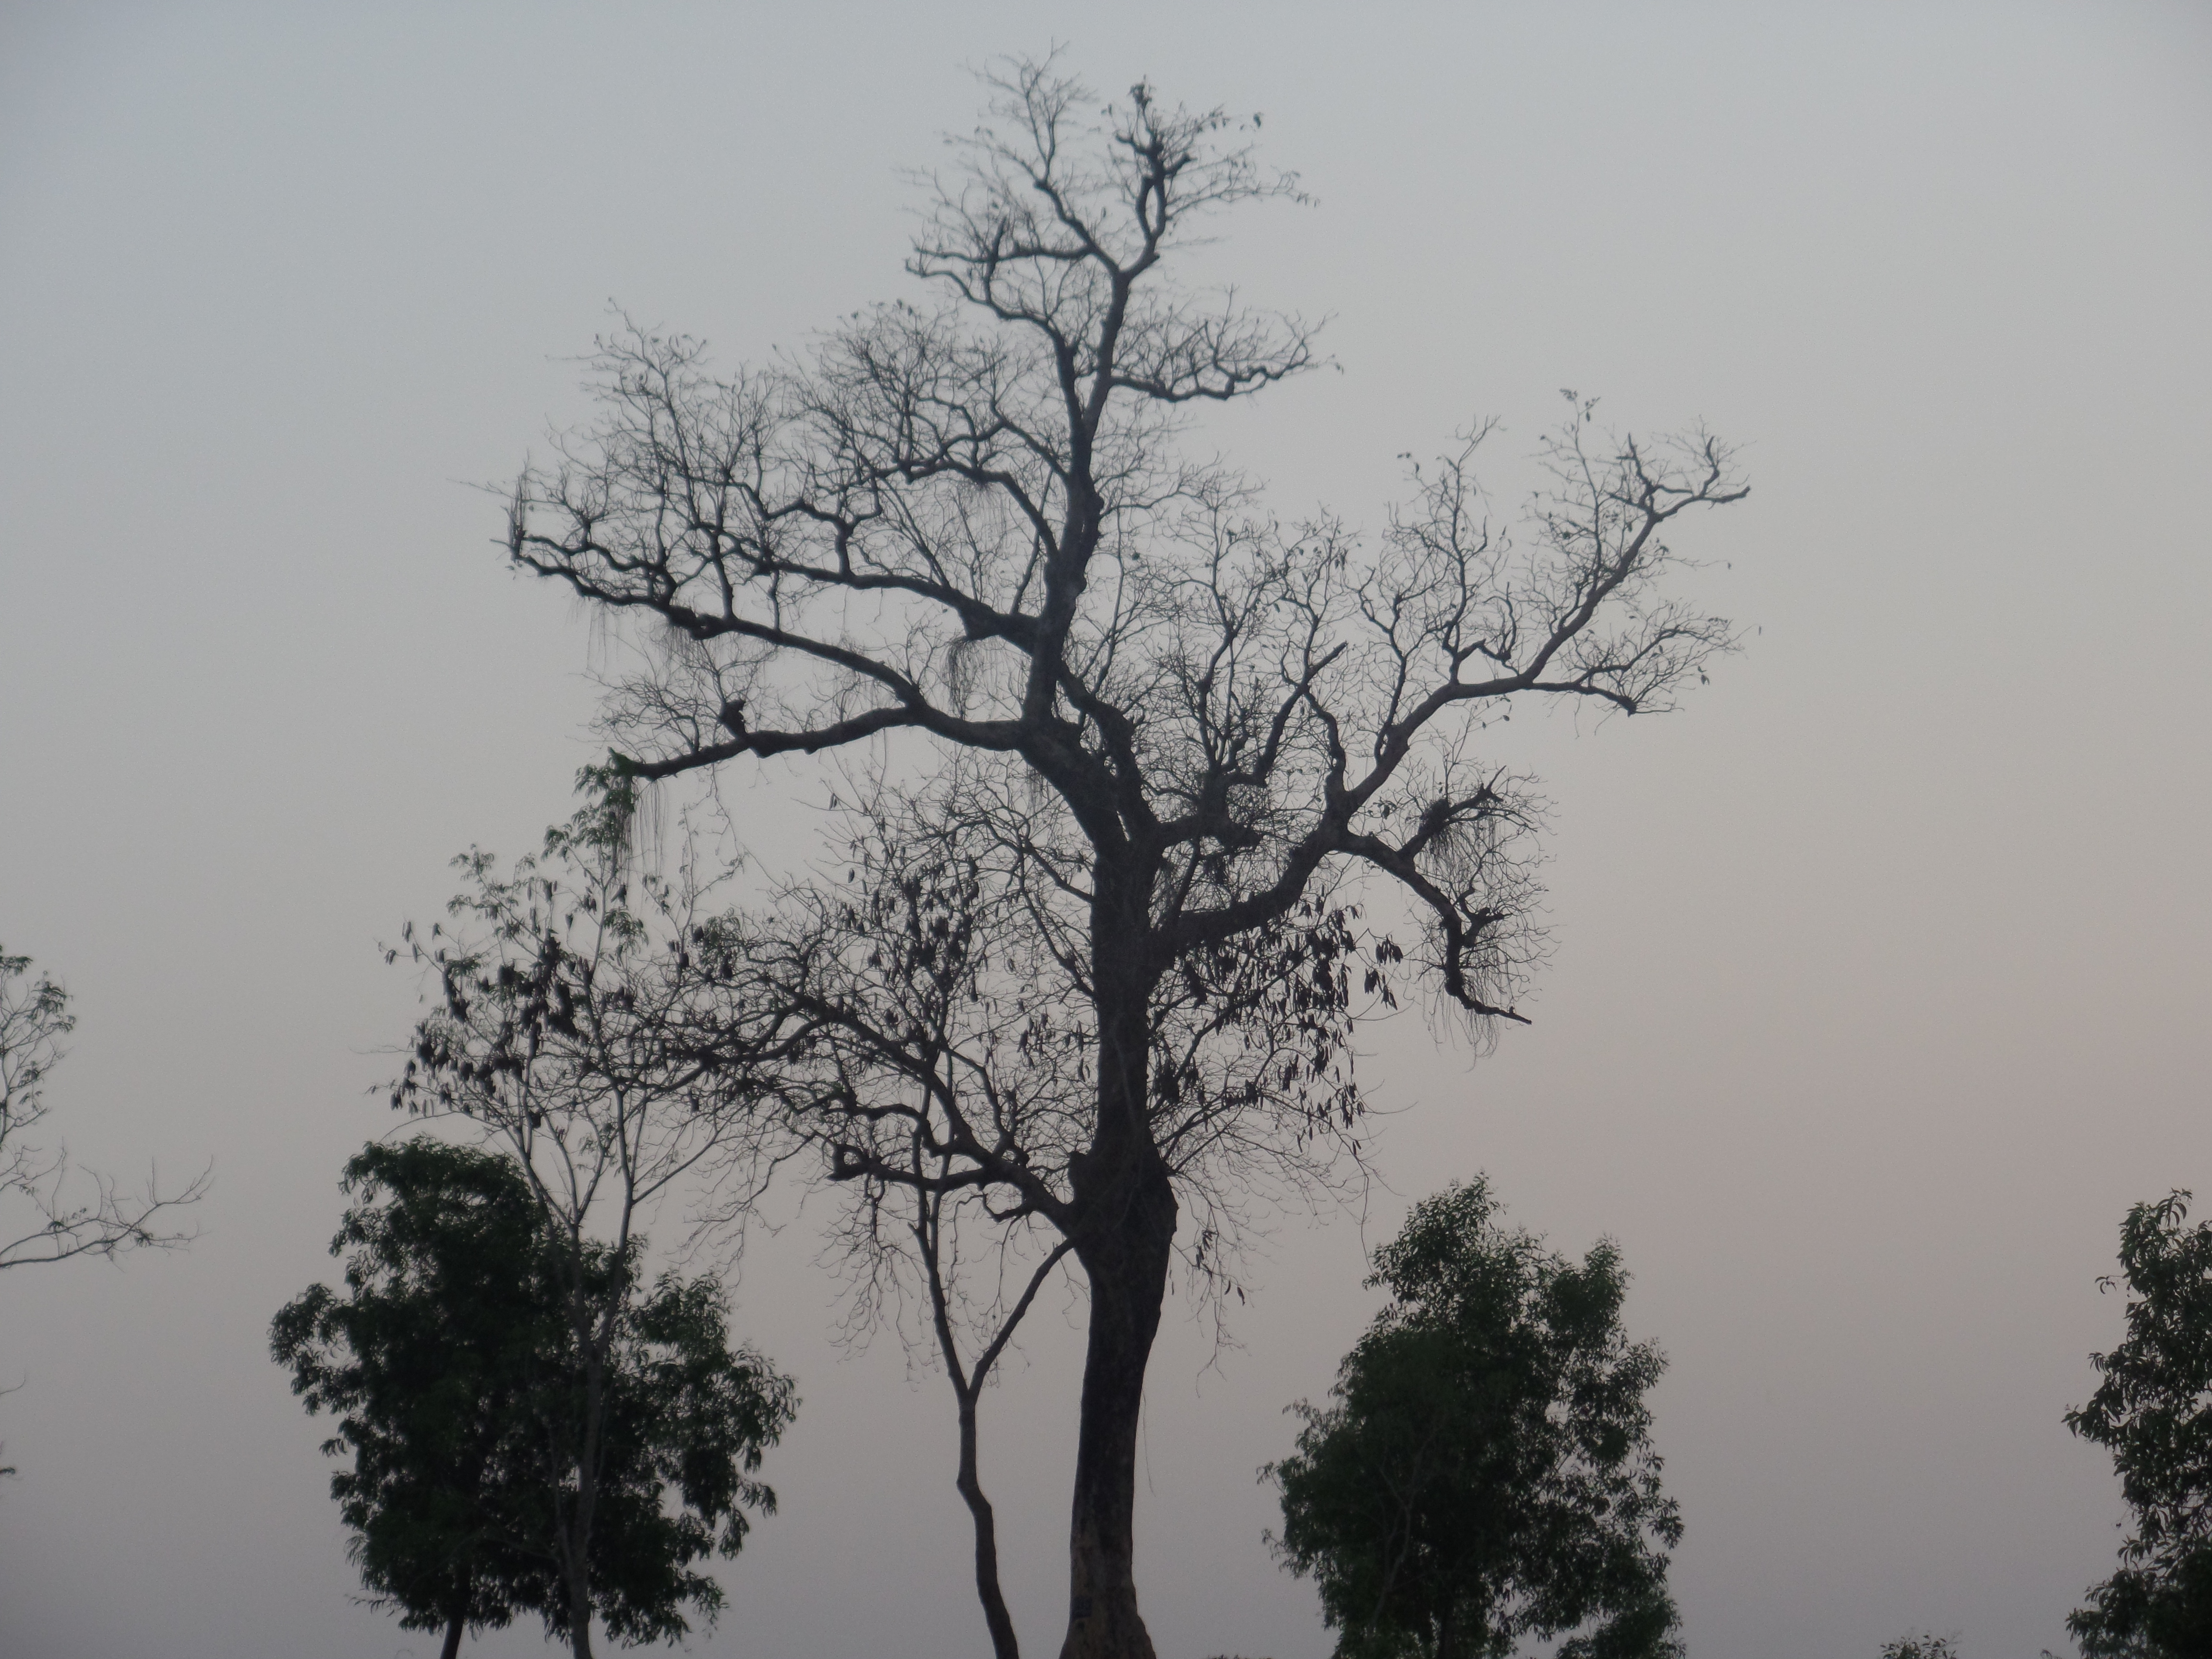
\includegraphics[width=0.6\textwidth]{figures/tree.jpg}\\
		\hspace*{15pt}\hbox{\scriptsize Image By:\thinspace{\itshape George achik}}
		% https://commons.wikimedia.org/wiki/File:Last_summer_time_tree_and_evening_time,_In_Srimongol,_Bangladesh.jpg
	\end{center}
\end{frame}

\begin{frame}
	\frametitle{Properties}
	\begin{columns}
		\column{0.405\textwidth}
			\begin{tikzpicture}[
				level distance = 2.5em,
				level 1/.style={sibling distance=9em},
				level 2/.style={sibling distance=4.5em},
				level 3/.style={sibling distance=2.25em},
			]
			\node[ellipse,onslide=<5>{draw=red}] (t1) {\alert<1,6>{root}}
				child { node[ellipse] {\alert<2,4,5>{child 1}}
					child { node[ellipse] {\alert<3,5>{leaf 1}}}
				}
				child { node[ellipse] {\alert<2,4,5,6>{child 2}}
					child { node[ellipse] {\alert<3,5>{leaf 2}}}
					child { node[ellipse,onslide=<6>{draw=red}] {\alert<3,5>{leaf 3}}}
					child { node[ellipse] {\alert<3,5>{leaf 4}}}
				};
			\end{tikzpicture}
		\column{0.555\textwidth}
		\begin{itemize}
			\item The \textit{root node} is the node that has no \textit{parent}.
				\pause
			\item A node can have \textit{children}.
				\pause
			\item A node without children is called a \textit{leaf}.
				\pause
			\item Two nodes with the same \textit{parent} are \textit{siblings}.
				\pause
			\item \textit{Descendants} are found by repeatedly following child-relations.
				\pause
			\item \textit{Ancestors} are found by repeatedly following parent-relations.
		\end{itemize}
	\end{columns}
\end{frame}

\begin{frame}
	\frametitle{Quick check}
	
	\begin{columns}
		\column{0.405\textwidth}
			\begin{tikzpicture}[
				level distance = 2.5em,
				level 1/.style={sibling distance=2em},
				level 2/.style={sibling distance=4.5em},
				level 3/.style={sibling distance=2.25em},
			]
			\node[ellipse] (t1) {r}
				child { node[ellipse] {k}
					child { node[ellipse] {d}}
				}
				child { node[ellipse] {a} }
				child { node[ellipse] {b} }
				child { node[ellipse] {e} 
					child { node[ellipse] {g} }
					child { node[ellipse] {h}
						child { node[ellipse] {i}}
					}
				}
				child { node[ellipse] {f} };
			\end{tikzpicture}
		\column{0.555\textwidth}
		\pause
			\begin{questionblock}{Let's see if that was a clear}
				Let $c(v)$ be the set of children of $v$.\\
				Let $d(v)$ be the set of descendants of $v$.\\
				Let $s(v)$ be the set of siblings of $v$.\\
				Let $a(v)$ be the set of ancestors of $v$.\\
				Let $p(v)$ be the parent of $v$.\\
				What is: $|c(k)| + |d(p(g))| + \sum\limits_{v \in a(h)} |s(v)|$?
				\begin{multicols}{2}
				\begin{enumerate}[A.]
					\item 4
					\item 8
					\item 12
					\item I don't know
				\end{enumerate}
			\end{multicols}
			\end{questionblock}
	\end{columns}
	\pause
	\vspace{-5pt}
	\begin{answerblock}{Arithmetic time}
		$c(k) = \{d\}$, $p(g) = e$, $d(e) = \{g,h,i\}$, $a(h) = \{r,e\}$, $s(r) = \emptyset$, $s(e) = \{k,a,b,f\}$. So the
		final answer is: $1+3+4=8$.
	\end{answerblock}
\end{frame}

\section{Tree properties pt2}
\label{sec:tree_functions}

\begin{frame}
	\frametitle{Tree properties pt2}
	\begin{center}
		\includegraphics[width=0.6\textwidth]{figures/stick.png}\\
		\hspace*{15pt}\hbox{\scriptsize Image By:\thinspace{\itshape Edfrank01}}
		% https://commons.wikimedia.org/wiki/File:Stick_measurement.png
	\end{center}
\end{frame}

\begin{frame}
	\frametitle{Depth of a node}

	\begin{columns}
		\column{0.405\textwidth}
			\begin{tikzpicture}[
				level distance = 2.5em,
				level 1/.style={sibling distance=9em},
				level 2/.style={sibling distance=4.5em},
				level 3/.style={sibling distance=2.25em},
			]
			\node[ellipse] (t1) {root}
				child { node[ellipse]   {child 1}
					child { node[ellipse] {l1}}
				}
				child { node[ellipse]   {child 2}
					child { node[ellipse] {l2}}
					child { node[ellipse] {l3}}
					child { node[ellipse] {l4}}
				};
			\end{tikzpicture}
		\column{0.555\textwidth}
		\begin{itemize}
			\item The \textit{depth} of a \alert<5->{node} is the distance to the root.
				\pause
			\item So depth(root) = 0.
			\item And depth(l2) = 2.
				\pause
			\item The \textit{height} of a \alert<5->{tree} is the length of the longest path from root to leaf.
				\pause
			\item So the height of this tree is 3.
				\pause
			\item Note: Every book/author has their own definition of these things! Including our book :(
		\end{itemize}
	\end{columns}
	
\end{frame}

\begin{frame}
	\frametitle{Depth of a node}

	\begin{columns}
		\column{0.405\textwidth}
			\begin{tikzpicture}[
				level distance = 2.5em,
				level 1/.style={sibling distance=9em},
				level 2/.style={sibling distance=4.5em},
				level 3/.style={sibling distance=2.25em},
			]
			\node[ellipse] (t1) {root}
				child { node[ellipse]   {child 1}
					child { node[ellipse] {l1}}
				}
				child { node[ellipse]   {child 2}
					child { node[ellipse] {l2}}
					child { node[ellipse] {l3}}
					child { node[ellipse] {l4}}
				};
			\end{tikzpicture}
		\column{0.555\textwidth}
		\begin{questionblock}{Alternative definition for height}
			How can we also describe the tree height of a tree $T$?
			\pause
			\begin{enumerate}[A.]
				\item $\max\limits_{v\in T}({\textit{depth}(v)})-1$
				\item $\max\limits_{v\in T}({\textit{depth}(v)})$
				\item $\max\limits_{v\in T}({\textit{depth}(v)})+1$
			\end{enumerate}
		\end{questionblock}
	\end{columns}
	\pause
	\begin{answerblock}{A tree of height one}
		Remember that a tree of height one is just the root, which is at depth $0$. So it cannot be A or B.\\
		Then remember that depth is the distance, but height is the length of the path. These differ by 1, so C is the right
		answer.\\
		Our book uses $B$ :( 
	\end{answerblock}
\end{frame}

\begin{frame}
	\frametitle{An implementation}
	
	\begin{questionblock}{How do we implement this?}
		How can we implement such a tree structure?
	\end{questionblock}
	\pause
	\begin{answerblock}{Just like a DLL, only different}
		By using nodes that are \textit{linked} together to form a tree!
	\end{answerblock}
	\pause
	\begin{columns}[t]
		\column{0.535\textwidth}
	\lstinputlisting{code/tree.py}
			
		\column{0.505\textwidth}
	\lstinputlisting{code/treenode.py}
			
	\end{columns}
\end{frame}

\begin{frame}
	\frametitle{Now we can create functions!}
	\begin{questionblock}{Implementing functionality}
		What kind of \textit{programming paradigm} will we use to implement tree functions?
	\end{questionblock}
	\pause
	\begin{answerblock}{See the contents of this box}
		See the title of this box.
	\end{answerblock}
\end{frame}

\begin{frame}
	\frametitle{Node Depth}
		\begin{exampleblock}{Example: Node depth}
			Find the depth of a node is easy if we know the depth of the parent.
		\end{exampleblock}	
		\pause
		\lstinputlisting{code/nodedepth.py}
\end{frame}

\begin{frame}
	\frametitle{Tree Height}
		\begin{exampleblock}{Example: Tree height}
			The height of the tree is the max depth + 1! 	
		\end{exampleblock}	
		\pause
		\lstinputlisting{code/treeheight.py}
\end{frame}

\begin{frame}
	\frametitle{Getting all the leaves}
	\begin{questionblock}{It's autumn time}
		How can we get all the leaves from a tree?
	\end{questionblock}
		\pause
		\lstinputlisting{code/treeleaves.py}
\end{frame}

\begin{frame}
	\frametitle{The full ADT}
		\begin{alertblock}{A Tree ADT}
			Different implementations of trees, give you different ADTs.\\
			The book uses one which is \textit{position}-focused.\\
			The properties are always the same, just the functions and how to call them can be different.
		\end{alertblock}	
\end{frame}

\begin{frame}
	\frametitle{Alternative implementation}
		\begin{block}{An observation}
			Every node in a tree, is the root to a subtree!
		\end{block}	
		\pause
		\begin{columns}
			\column{0.455\textwidth}
				
			\begin{tikzpicture}[
				level distance = 2.5em,
				level 1/.style={sibling distance=9em},
				level 2/.style={sibling distance=4.5em},
				level 3/.style={sibling distance=2.25em},
			]
			\node[ellipse] (t1) {root}
				child { node[ellipse]   {child 1}
					child { node[ellipse] {l1}}
				}
				child { node[ellipse,onslide=<3>{draw=red}]   {child 2}
					child { node[ellipse] {\alert<3>{l2}}}
					child { node[ellipse] {\alert<3>{l3}}}
					child { node[ellipse] {\alert<3>{l4}}
						child { node[ellipse] {\alert<3>{l5}}}
						child { node[ellipse] {\alert<3>{l6}}}
					}
				};
			\end{tikzpicture}
			\pause
			\column{0.455\textwidth}
				\begin{exampleblock}{A subtree}
					In the example on the right, child 2 is the root of the subtree drawn in red.
				\end{exampleblock}	
		\end{columns}
\end{frame}

\begin{frame}
	\frametitle{Alternative implementation}
		\begin{block}{Thinking of all nodes as trees}
			By implementing it like this, we have no need for \texttt{TreeNode}s. All nodes are just \texttt{Tree}s!
		\end{block}	

		\lstinputlisting{code/tree_alt.py}
\end{frame}

\begin{frame}
	\frametitle{Alternative implementation: Tree Height}
	\begin{questionblock}{What do we do?}
		How do we determine the height in this set-up?
	\end{questionblock}
	\pause
	\lstinputlisting{code/tree_alt_height.py}
\end{frame}

\begin{frame}
	\frametitle{Why have one implementation over the other?}

	\begin{questionblock}{Which is better?}
		Which implementation should you use?
	\end{questionblock}
	\pause
	\begin{answerblock}{IT DEEP ENDS}
		It depends of course ;)\\
		What information do you need to store for your use case?
	\end{answerblock}
	
\end{frame}



\section{Intermezzo}
\label{sec:intermezzo}

\begin{frame}
	\frametitle{Intermezzo: Databases}

	$\left. 
		\begin{array}{rl} 
			\scriptstyle\mathtt{UPDATE~clause} & \{ \mathtt{UPDATE\ country} \\
				\scriptstyle\mathtt{SET~clause} & \{ \mathtt{SET\ population =~} \overbrace{\mathtt{population + 1}}^\mathtt{expression} \\ 
				\scriptstyle\mathtt{WHERE~clause} & \{ \mathtt{WHERE}\ \underbrace{\mathtt{name =} \underbrace{\mathtt{'USA'}}_{expression}}_{predicate};
		\end{array}
	\right\} \scriptstyle\texttt{statement}$
\end{frame}

\begin{frame}
	\frametitle{Large-scale databases}
	\begin{itemize}
		\item Databases come in all shapes and sizes.
			\pause
		\item Many are tuple-based (or \textit{relational}).
			\pause
		\item And these things can grow very large! Millions of records.
			\pause
		\item So binary searching, instead of linear searching can help a lot!
			\pause
		\item To this end they use B-trees (generalised binary search trees).
			\pause
		\item Searching goes down to 30~ish comparisons instead of a million.
	\end{itemize}
	
\end{frame}

\begin{frame}
	\frametitle{Btree advantages}
	\framesubtitle{\url{https://en.wikipedia.org/wiki/B-tree\#Advantages\_of\_B-tree_usage_for_databases}}
	\begin{itemize}
		\item keeps keys in sorted order for sequential traversing
		\item uses a hierarchical index to minimise the number of disk reads
		\item uses partially full blocks to speed insertions and deletions
		\item keeps the index balanced with a recursive algorithm
	\end{itemize}
	\pause
	\begin{block}{TL;DR}
		It helps :D
	\end{block}	
\end{frame}

\section{Time complexities}
\label{sec:time_complexities}

\begin{frame}
	\frametitle{How long does this all take?}
	
	\begin{center}
		\includegraphics[width=0.6\textwidth]{figures/tree_age.jpg}\\
		\hspace*{15pt}\hbox{\scriptsize Image By:\thinspace{\itshape Garry Knight}}
		% https://www.flickr.com/photos/garryknight/3829280573
	\end{center}
\end{frame}

\begin{frame}
	\frametitle{Expressing time complexity}
	\begin{questionblock}{How can we express the time of Tree operations?}
		For operations like \texttt{height} and \texttt{depth} what is the time complexity?
	\end{questionblock}
	\pause
		\begin{block}{Two parameters}
			For functions on trees, we consider two parameters:
			\begin{itemize}
				\item $n$ the number of nodes in the tree.
				\item $h$ the height of the tree.
			\end{itemize}
		\end{block}	
\end{frame}

\begin{frame}
	\frametitle{Alternative implementation: Node Depth}
	
	\lstinputlisting{code/tree_alt_depth.py}
	\begin{questionblock}{What do we do?}
		What is the time complexity of this function?\\
		Note: this uses the implementation wher every node is a subtree itself.
		\only<2>{
		\begin{multicols}{2}
			\begin{enumerate}[A.]
				\item $\Theta(h)$
				\item $\Theta(h^2)$
				\item $\Theta(n)$
				\item $\Theta(n^2)$
			\end{enumerate}
		\end{multicols}
	}
	\end{questionblock}
	\only<3>{
	\begin{answerblock}{Like sending a hobbit up a tree}
		We only consider one path straight to the top, so this is $O(h)$.
	\end{answerblock}
}
\end{frame}

\begin{frame}
	\frametitle{Alternative implementation: Tree Height}
	\lstinputlisting{code/tree_alt_height.py}
	\begin{questionblock}{What do we do?}
		What is the time complexity of this function?\\
		Note: this uses the implementation wher every node is a subtree itself.
		\only<2>{
		\begin{multicols}{2}
			\begin{enumerate}[A.]
				\item $\Theta(h)$
				\item $\Theta(h^2)$
				\item $\Theta(n)$
				\item $\Theta(n^2)$
			\end{enumerate}
		\end{multicols}
	}
	\end{questionblock}
	\only<3>{
	\begin{answerblock}{Some kind of irony}
		Worst case we need to check all nodes, so $O(n)$ to determine $h$.
	\end{answerblock}
}
\end{frame}



\section{Binary Trees}
\label{sec:binary_trees}


\begin{frame}
	\frametitle{Binary Trees}
	\framesubtitle{Tikz taken from: \url{http://texample.net/tikz/examples/red-black-tree/}}
	\begin{center}
			\begin{tikzpicture}[->,>=stealth',level/.style={sibling distance = 4cm,
		  level distance = 1.5cm},
			  treenode/.style = {align=center, inner sep=0pt, text centered,
		    font=\sffamily},
		  arn_n/.style = {treenode, circle, white, font=\sffamily\bfseries, draw=black,
		    fill=black, text width=1.5em},% arbre rouge noir, noeud noir
		  arn_r/.style = {treenode, circle, red, draw=red,
		    text width=1.5em, very thick},% arbre rouge noir, noeud rouge
		  arn_x/.style = {treenode, rectangle, draw=black,
		    minimum width=0.5em, minimum height=0.5em}% arbre rouge noir, nil
			]
			\node [arn_n] {33}
    child{ node [arn_r] {15}
            child{ node [arn_n] {10}
            	child{ node [arn_r] {5} edge from parent node[above left]
                         {$x$}} %for a named pointer
							child{ node [arn_x] {}}
            }
            child{ node [arn_n] {20}
							child{ node [arn_r] {18}}
							child{ node [arn_x] {}}
            }
    }
    child{ node [arn_r] {47}
            child{ node [arn_n] {38}
							child{ node [arn_r] {36}}
							child{ node [arn_r] {39}}
            }
            child{ node [arn_n] {51}
							child{ node [arn_r] {49}}
							child{ node [arn_x] {}}
            }
		}
;
\end{tikzpicture}
	\end{center}
	
\end{frame}

\begin{frame}
	\frametitle{Binary Trees}
	\framesubtitle{All we need}

		\begin{block}{Binary Trees}
			\begin{itemize}
				\item Every node has at most 2 children.
					\pause
				\item One \textit{left} child and one \textit{right} child.
			\end{itemize}
		\pause
		A binary tree is \textit{proper} or \textit{full} if all nodes have either 0 or 2 children.
		\end{block}	

		\pause
		\begin{columns}
			\column{0.455\textwidth}
				
			\begin{tikzpicture}[
				level distance = 2.5em,
				level 1/.style={sibling distance=9em},
				level 2/.style={sibling distance=4.5em},
				level 3/.style={sibling distance=2.25em},
			]
			\node[ellipse] (t1) {root}
				child { node[ellipse]   {child 1}
					child { node[ellipse] {l1}}
					child { node[ellipse] {l2}}
				}
				child { node[ellipse]   {child 2}
					child { node[ellipse] {l3}}
					child { node[ellipse] {l4}
						child { node[ellipse] {l5}}
						child { node[ellipse] {l6}}
					}
				};
			\end{tikzpicture}
			\column{0.455\textwidth}
				
			\begin{questionblock}{Is it full?}
				Is this tree full?
				\begin{enumerate}[A.]
					\item Yes
					\item No
					\item I don't know
				\end{enumerate}
			\end{questionblock}
		\end{columns}
\end{frame}

\begin{frame}
	\frametitle{All kinds of fun properties!}
	
		\begin{block}{Many interesting properties}
			There are many interesting relations in binary trees, between the number of internal nodes vs leaves, height, etc.	
		\end{block}	
		\pause
		\begin{exampleblock}{Just one example}
			There is always one more leaf than there are internal nodes in a full binary tree.
		\end{exampleblock}	
\end{frame}

\section{Traversals}
\label{sec:traversals}

\begin{frame}
	\frametitle{Tree traversals}
	\framesubtitle{Walking through our tree}

	\begin{center}
		\includegraphics[trim={0 4cm 0 4cm},clip, width=0.65\textwidth]{figures/bearcub.jpg}\\
		\hspace*{15pt}\hbox{\scriptsize Image By:\thinspace{\itshape Skeeze}}
		% https://pixabay.com/photos/bear-cub-brown-climbing-tree-1576559/
	\end{center}

\end{frame}

\begin{frame}
	\frametitle{Iterating over the nodes}
	
		\begin{block}{Finding all the nodes}
			If you want to iterate over the tree, you can do so in many different orders. Three common ones for binary trees are:
			\begin{itemize}
				\item Pre-order traversal
				\item In-order traversal
				\item Post-order traversal
			\end{itemize}
		\end{block}	
\end{frame}

\begin{frame}
	\frametitle{Pre-order traversal}
	\begin{overlayarea}{\textwidth}{\textheight}
			\begin{columns}
				\column{0.455\textwidth}
				\begin{itemize}
					\item First give the value of the current node.
					\item Then a pre-order traversal of the left child.
					\item Then a pre-order traversal of the right child.
				\end{itemize}
				\column{0.455\textwidth}
				\pause
					\begin{tikzpicture}[
						level distance = 2.5em,
						level 1/.style={sibling distance=9em},
						level 2/.style={sibling distance=4.5em},
						level 3/.style={sibling distance=2.25em},
					]
					\node[ellipse,onslide=<3>{draw=red}] (t1) {\alert<3>{1}}
					child { node[ellipse,onslide=<4>{draw=red}]   {\alert<4>{2}}
						child { node[ellipse,onslide=<5>{draw=red}] {\alert<5>{3}}}
						}
						child { node[ellipse,onslide=<6>{draw=red}]   {\alert<6>{4}}
							child { node[ellipse,onslide=<7>{draw=red}] {\alert<7>{5}}}
							child { node[ellipse,onslide=<8>{draw=red}] {\alert<8>{6}}
								child { node[ellipse,onslide=<9>{draw=red}] {\alert<9>{7}}}
								child { node[ellipse,onslide=<10>{draw=red}] {\alert<10>{8}}}
							}
						};
					\end{tikzpicture}
			\end{columns}
			\only<11>{
			\begin{exampleblock}{Amsterdam, Rotterdam, no not that kind of topology!}
				Gives us a \textit{topological} order of the tree.\\
				If all nodes represent jobs, and job $i$ depends on it's parent job $p$ then this gives us an order in which we can
				do all jobs, satisfying these dependencies.
			\end{exampleblock}
		}
	\end{overlayarea}
\end{frame}

\begin{frame}
	\frametitle{In-order traversal}
	\begin{overlayarea}{\textwidth}{\textheight}
			\begin{columns}
				\column{0.455\textwidth}
				\begin{itemize}
					\item First an in-order traversal of the left child.
					\item Then give the value of the current node.
					\item Then an in-order traversal of the right child.
				\end{itemize}
				\column{0.455\textwidth}
					\begin{tikzpicture}[
						level distance = 2.5em,
						level 1/.style={sibling distance=9em},
						level 2/.style={sibling distance=4.5em},
						level 3/.style={sibling distance=2.25em},
					]
					\node[ellipse,onslide=<5>{draw=red}] (t1) {\alert<5>{1}}
					child { node[ellipse,onslide=<4>{draw=red}]   {\alert<4>{2}}
						child { node[ellipse,onslide=<3>{draw=red}] {\alert<3>{3}}}
						}
						child { node[ellipse,onslide=<7>{draw=red}]   {\alert<7>{4}}
							child { node[ellipse,onslide=<6>{draw=red}] {\alert<6>{5}}}
							child { node[ellipse,onslide=<9>{draw=red}] {\alert<9>{6}}
								child { node[ellipse,onslide=<8>{draw=red}] {\alert<8>{7}}}
								child { node[ellipse,onslide=<10>{draw=red}] {\alert<10>{8}}}
							}
						};
					\end{tikzpicture}
			\end{columns}
			\only<2>{
				\begin{questionblock}{In-order}
				What is the order of nodes now?
				\begin{multicols}{2}
					\begin{enumerate}[A.]
						\item 1,2,3,4,5,6,7,8
						\item 3,2,1,5,4,7,6,8
						\item 3,2,8,7,6,5,4,1
						\item 8,7,6,5,4,3,2,1
					\end{enumerate}
				\end{multicols}
			\end{questionblock}
		}
			\only<11>{
				\begin{exampleblock}{We'll save that for tomorrow}
				We will see an example for this tomrrow!
			\end{exampleblock}
		}
	\end{overlayarea}
\end{frame}

\begin{frame}
	\frametitle{Post-order traversal}
	\begin{overlayarea}{\textwidth}{\textheight}
			\begin{columns}
				\column{0.455\textwidth}
				\begin{itemize}
					\item First a post-order traversal of the left child.
					\item Then a post-order traversal of the right child.
					\item Then give the value of the current node.
				\end{itemize}
				\column{0.455\textwidth}
					\begin{tikzpicture}[
						level distance = 2.5em,
						level 1/.style={sibling distance=9em},
						level 2/.style={sibling distance=4.5em},
						level 3/.style={sibling distance=2.25em},
					]
					\node[ellipse,onslide=<10>{draw=red}] (t1) {\alert<10>{1}}
					child { node[ellipse,onslide=<4>{draw=red}]   {\alert<4>{2}}
						child { node[ellipse,onslide=<3>{draw=red}] {\alert<3>{3}}}
						}
						child { node[ellipse,onslide=<9>{draw=red}]   {\alert<9>{4}}
							child { node[ellipse,onslide=<5>{draw=red}] {\alert<5>{5}}}
							child { node[ellipse,onslide=<8>{draw=red}] {\alert<8>{6}}
								child { node[ellipse,onslide=<6>{draw=red}] {\alert<6>{7}}}
								child { node[ellipse,onslide=<7>{draw=red}] {\alert<7>{8}}}
							}
						};
					\end{tikzpicture}
			\end{columns}
			\only<2>{
				\begin{questionblock}{Post-order}
				What is the order of nodes now?
				\begin{multicols}{2}
					\begin{enumerate}[A.]
						\item 1,2,3,4,5,6,7,8
						\item 3,2,5,8,7,6,4,1
						\item 3,2,8,7,6,5,4,1
						\item 8,7,6,5,4,3,2,1
					\end{enumerate}
				\end{multicols}
			\end{questionblock}
		}
			\only<11>{
				\begin{exampleblock}{I didn't mean to sound so dark :(}
				Used to delete a tree (first delete your children, before deleting yourself).
			\end{exampleblock}
		}
	\end{overlayarea}
\end{frame}

\section{Parsing math expressions Part 2}
\label{sec:parsing_math_expressions}

\begin{frame}
	\frametitle{A parse tree}
	\begin{columns}
		\column{0.555\textwidth}
  \begin{tikzpicture}[
    level distance = 2.5em,
    level 1/.style={sibling distance=11em},
    level 2/.style={sibling distance=4.5em},
    level 3/.style={sibling distance=2.25em},
  ]
  \node[ellipse] (t1) {/}
    child { node[ellipse] {$\times$}
      child { node[ellipse] {-} 
				child { node[ellipse] {8}} 
				child { node[ellipse] {$\sqrt{\invisible{x}}$}
					child { node[ellipse] {16}}}}
			child { node[ellipse] {2}}}
    child { node[ellipse] {+}
			child { node[ellipse] {-}
				child { node[ellipse] {4}}}
			child { node[ellipse] {3}}};
  \end{tikzpicture}\\
		\column{0.355\textwidth}
		\begin{questionblock}{What order?}
			In what order should we evaluate this parse tree to get the right answer?
			\begin{enumerate}[A.]
				\item Pre-order
				\item In-order
				\item Post-order
				\item Something else
			\end{enumerate}
		\end{questionblock}
	\end{columns}
	\pause
	\begin{answerblock}{Post-order}
		First find the two subresults, then combine them!
	\end{answerblock}
\end{frame}

\begin{frame}
	\frametitle{A basic implementation}
	
	\lstinputlisting{code/parsemath.py}
\end{frame}


\begin{frame}
	\frametitle{You are here.}
	\begin{block}{The course so far}
		\begin{itemize}
			\item Time and Space Complexity
			\item Array-based vs Linked Lists
		\end{itemize}
	\end{block}
	\pause
	\begin{exampleblock}{Today's content}
		\begin{itemize}
			\item Stacks \& Queues
			\item Example: Parsing LaTeX
			\item An experiment (of great scientific value)
		\end{itemize}
	\end{exampleblock}
	\pause
	\begin{block}{The future}
		\begin{itemize}
			\item Next time: Sorting
			\item Trees, Graphs...
			\item P vs NP, and much more!
		\end{itemize}
	\end{block}
\end{frame}

\begin{frame}
	\frametitle{Homework for this week}
	\begin{itemize}[<+->]
		\item \alert{After} today's lecture: read the Chapter 8.
		\item \alert{Before} Friday, check out the example exam (so that you can ask questions).
		\item \alert{Before} Sunday, do the homework :)
	\end{itemize}
\end{frame}

\begin{frame}
	\frametitle{Mudcards}
	\framesubtitle{\url{https://www.delta.tudelft.nl/article/column-van-koelkasten-kranen-en-college}}

	\begin{block}{Based on a column by Bob van Vliet}
		\begin{itemize}
			\item At the end of every lecture, a short (2-question) survey.
			\item Tell me one thing you liked.
			\item And one thing you didn't like.
			\item Be concrete, be specific!
		\end{itemize}
	\end{block}
\end{frame}



\frame{\titlepage}

\end{document}
